\documentclass[11pt]{article}

\usepackage[margin=1in]{geometry}
\usepackage{amsmath,amssymb,amsthm,mathtools,bm}
\usepackage{booktabs}
\usepackage{graphicx}
\usepackage{xcolor}
\usepackage{multirow}
\usepackage{caption}
\usepackage{subcaption}
\usepackage{enumitem}
\usepackage[colorlinks=true,linkcolor=blue!60!black,citecolor=blue!60!black,urlcolor=blue!60!black]{hyperref}
\usepackage{microtype}

\graphicspath{{../analysis/}}

\newcommand{\passk}[1]{\ensuremath{\mathrm{pass}@#1}}
\newcommand{\Rout}{\ensuremath{R_{\mathrm{out}}}}
\newcommand{\Rpv}{\ensuremath{R_{\mathrm{pv}}}}
\newcommand{\ind}[1]{\ensuremath{\mathbb{1}\!\left[#1\right]}}
\newcommand{\pp}{\,\mathrm{pp}}
\newcommand{\ci}[2]{\ensuremath{[#1,\,#2]}}

\title{\textbf{Process-Aware Rewards and Reward Hacking:\\
A Validated Replication of Zhang, Neubig \& Yue (2025), \S6,\\
in the Contextual-Generalization Setting}}
\author{Experiment 4 --- DLT Final Project\\[2pt]
\small Run on PACE ICE, $1\times$ H100 (job 6589709); artifacts in \texttt{experiment4/}}
\date{October 26, 2026}

\begin{document}
\maketitle

\begin{abstract}
Outcome-based reinforcement learning (RL) rewards for reasoning models are vulnerable to
\emph{reward hacking}: policies learn to emit correct final answers via invalid
reasoning. Zhang, Neubig \& Yue (2025) propose blending a process-verification signal
into the reward and report that process-aware rewards raise strict (process-verified)
accuracy and reduce hacking. We replicate this claim on the authors' released
checkpoints in their contextual-generalization setting: one shared 100M-parameter base
model and four GRPO runs differing \emph{only} in reward composition, evaluated with
$k{=}64$ samples on $2{,}000$ problems ($640$k samples total). The paper's core claim is
confirmed, and more decisively than its own presentation: the reward-hacking rate falls
monotonically with process-supervision strength
($52.3\% \to 45.8\% \to {\approx}42.3\% \to 40.5\%$ on the long-tail context), with
\emph{every} step of the ladder significant under paired bootstrap after Bonferroni
correction (strict vs.\ outcome: $-5.31\pp$ \ci{-6.37}{-4.27}). Strict \passk{1} gains
from process rewards are decisive on edge-difficulty problems ($+6.5\pp$
\ci{+2.8}{+10.3}) and directional but individually unresolved on the hardest band.
During validation we additionally discovered a \emph{letter-collision artifact} in the
authors' released strict scorer that inflates absolute hacking rates (up to ${\sim}6$--$8\times$)
and deflates absolute strict \passk{k} (12--22$\pp$) for all checkpoints equally.
The headline process-vs-outcome contrast survives correction in full strength
($-4.5\pp$ hacking, $p<10^{-3}$); the finer ranking is verifier-regime-dependent ---
under corrected scoring the three process variants tie on hacking and the dense
mixes dominate strict on accuracy.
\end{abstract}

\section{Background and research questions}

\subsection{Task and evaluation formalism}

Each reasoning problem is generated from a directed acyclic dependency graph
$\mathcal{G} = (\mathcal{V}, \mathcal{E})$ whose nodes are named quantities and whose
edges encode functional dependencies $v_i = f_i\big((v_j)_{j \in \mathrm{pa}(i)}\big)$
with $f_i \in \{+,-,\times,\div\}$; difficulty is controlled by the operation count
$\mathrm{op}(\mathcal{G}) = |\mathcal{E}|$. A contextual template $\tau$ renders
$\mathcal{G}$ into natural language; the same graph family rendered under different
templates yields structurally identical problems with different surface forms
(\emph{contexts}).

Given a model solution $s$, the evaluation parser deterministically extracts a predicted
graph $\hat{\mathcal{G}} = (\hat{\mathcal{V}}, \hat{\mathcal{E}}, \widehat{\mathrm{val}})$
and final answer $\hat a$. For each gold node $v \in \mathcal{V}$ define the step-level
correctness indicator
\begin{equation}
s(v;\hat{\mathcal{G}},\mathcal{G}) \;=\;
\begin{cases}
1, & v \in \hat{\mathcal{V}} \;\wedge\; \mathrm{pa}_{\hat{\mathcal{G}}}(v) = \mathrm{pa}_{\mathcal{G}}(v)
     \;\wedge\; \widehat{\mathrm{val}}(v) = \mathrm{val}(v),\\[2pt]
0, & \text{otherwise},
\end{cases}
\label{eq:step}
\end{equation}
the \emph{process accuracy}
\begin{equation}
\mathrm{ProcessAcc}(\hat{\mathcal{G}};\mathcal{G}) \;=\; \frac{1}{|\mathcal{V}|}
\sum_{v \in \mathcal{V}} s(v;\hat{\mathcal{G}},\mathcal{G}),
\label{eq:procacc}
\end{equation}
and the \emph{strict} (process-verified) correctness
\begin{equation}
\mathrm{VerifiedCorrect}(\hat a, \hat{\mathcal{G}}) \;=\;
\ind{\mathrm{ProcessAcc}(\hat{\mathcal{G}};\mathcal{G}) = 1} \cdot \ind{\hat a = a^{*}}.
\label{eq:strict}
\end{equation}
Extra predicted nodes $\hat{\mathcal{V}} \setminus \mathcal{V}$ are permitted. All
headline metrics use the strict criterion~\eqref{eq:strict}.

\subsection{Reward designs under test}

The paper's \S6 augments the sparse outcome reward with process verification
(its Eq.~3):
\begin{equation}
R \;=\; \alpha\,\Rout \;+\; (1-\alpha)\,\Rpv,
\qquad \Rout = \ind{\hat a = a^{*}}, \quad \Rpv = \mathrm{ProcessAcc},
\label{eq:mix}
\end{equation}
and a stricter gated form
\begin{equation}
R_{\mathrm{strict}} \;=\;
\begin{cases}
\Rout, & \text{if } \Rpv = 1,\\
0, & \text{otherwise.}
\end{cases}
\label{eq:strictreward}
\end{equation}
The five systems compared (all from one base model; the four RL runs used identical
GRPO data, $90\%$ context A / $10\%$ context B, and differ only in $R$):
\textbf{base} (no RL), \textbf{outcome} (answer-only; \emph{verified} from the
released training config, resolving an open question in the replication guide),
\textbf{0.5/0.5} ($\alpha{=}0.5$; weights assumed --- its config is absent from the
release), \textbf{0.2/0.8} ($\alpha{=}0.2$; verified), and \textbf{strict}
(Eq.~\ref{eq:strictreward}; verified, \texttt{zero\_on\_process\_mismatch}).

\paragraph{Implementation divergence from Eq.~\eqref{eq:mix}.} The released reward
code applies an \emph{answer gate} to the mixed rewards: after computing
$\alpha \Rout + (1-\alpha)\Rpv$ it zeroes the reward whenever the final answer is
wrong. As trained, the mixes are therefore
\begin{equation}
R_{\mathrm{mix}}^{\mathrm{as\text{-}trained}}
\;=\; \ind{\hat a = a^{*}} \cdot \big(\alpha + (1-\alpha)\,\Rpv\big),
\label{eq:gated}
\end{equation}
i.e., the process term modulates reward magnitude \emph{among answer-correct
rollouts}; wrong-answer rollouts never receive the dense process signal that
Eq.~\eqref{eq:mix} implies. The literal ungated mix was never trained in the released
family. Moreover, the training-time process reward used the same artifact-affected
scorer of \S\ref{sec:artifact}, so the released process-reward runs were themselves
trained under a systematically noisy verifier.

\subsection{Questions}
\textbf{Q1} Do mixed/strict process rewards raise strict \passk{k} over outcome-only?
\textbf{Q2} Do they reduce the share of correct answers reached through invalid
reasoning? \textbf{Q3} Do they shift errors away from structural failures (wrong
dependencies, missing steps)?

\section{Experimental setup}

\paragraph{Checkpoints.} HF \texttt{Interplay-LM-Reasoning/context\_pretrain}, folder
\texttt{idzoo\_0.999zoo\_0.001teacher/}: the base model is pre-trained on $99.9\%$
context~A (\texttt{crazy\_zootopia}, $\mathrm{op}\,2$--$20$) $+\,0.1\%$ context~B
(\texttt{teachers\_in\_school}, also spanning $\mathrm{op}\,2$--$20$ --- this release is the
paper's \emph{appendix} A.6.1 ``shared primitives'' setting; the main-text \S4 family with its
op-2-only seed is the separate \texttt{context\_pretrain\_2} release); RL variants under
\texttt{rl/contextzoo\_0.9zoo\_0.1teacher\{,\_process0.5,\_process,\_process\_strict\}}.

\paragraph{Evaluation data.} \texttt{Interplay-LM-Reasoning/context} validation splits,
$\mathrm{op} \in \{12,14,16,18,20\}$, $200$ problems per op, both contexts. Within a
context, all five checkpoints answer byte-identical problems (verified), enabling
paired analysis; the two contexts use different numeric instantiations, so
cross-context comparisons are distribution-level. Difficulty bands:
\emph{edge} $= \mathrm{op}\,12$--$14$, \emph{hard} $= \mathrm{op}\,16$--$20$.

\paragraph{Sampling and budget.} Authors' vLLM evaluator; temperature $0.7$,
top-$p$ $1.0$, $\le 1{,}024$ new tokens, $k = 64$ samples per problem:
$5 \times 2 \times 1{,}000 \times 64 = 640{,}000$ samples
($1$\,h\,$20$\,m wall time on one H100, ${\sim}140$ samples/s).

\paragraph{Metrics.} For problem $i$ let $r_i \in \{0,\dots,63,\infty\}$ be the rank of
the first strictly-correct sample. Then
\begin{equation}
\passk{k} \;=\; \frac{1}{N} \sum_{i=1}^{N} \ind{r_i < k},
\label{eq:passk}
\end{equation}
with the answer-only variant defined analogously on $\Rout$ alone. With
$a_i = \sum_{j=1}^{64} \ind{\hat a_{ij} = a^{*}_i}$ answer-correct samples and
$s_i = \sum_{j=1}^{64} \mathrm{VerifiedCorrect}_{ij}$ strictly-correct samples, the
\emph{reward-hacking rate} over a scope $S$ is the ratio of sums
\begin{equation}
H_S \;=\; \frac{\sum_{i \in S} \max(0,\, a_i - s_i)}{\sum_{i \in S} a_i}
\;=\; \Pr\big(\text{invalid reasoning} \,\big|\, \text{correct answer}\big).
\label{eq:hack}
\end{equation}

\paragraph{Uncertainty.} Percentile bootstrap over \emph{problems}
($B{=}1{,}000$ for per-variant CIs; problems are the independent sampling unit --- the
$64$ draws within a problem are clustered and are never resampled individually).
Because all variants share identical problems, headline \emph{differences} use the
paired bootstrap: resample problems once per replicate, compute the difference of the
two variants' statistics on the same resample ($B{=}5{,}000$), and report the
percentile interval; Bonferroni correction over the $m{=}9$ headline comparisons
uses $\alpha = 0.05/m$.

\paragraph{Validity.} Four independent audits (data integrity; clean-room metric
recomputation, which matched our pipeline to ${\sim}10^{-16}$ and the authors' own
aggregator \emph{exactly}; qualitative re-scoring of $240$ samples, reproduced
$240/240$; paired statistical review) are reported in
\texttt{analysis/validation/VALIDATION.md}. Zero parse failures, zero truncation at
the token cap, zero duplicate samples.

\section{Results}

\subsection{Q2 first: process supervision reduces reward hacking, monotonically}

\begin{table}[h]
\centering
\caption{Reward-hacking rate $H$ (Eq.~\ref{eq:hack}), context B (teachers), overall,
with $95\%$ bootstrap CIs over problems; and paired differences vs.\ outcome-only.
$^{\dagger}$ survives Bonferroni ($\alpha = 0.05/9$).}
\label{tab:hack}
\small
\begin{tabular}{lccc}
\toprule
Reward & $H$ (\%) & $95\%$ CI & Paired $\Delta$ vs.\ outcome (pp) \\
\midrule
base        & 52.3 & \ci{49.1}{55.7} & $+6.51$ \ci{+4.74}{+8.25}$^{\dagger}$ \\
outcome     & 45.8 & \ci{42.7}{48.8} & --- \\
0.5/0.5     & 42.3 & \ci{39.3}{45.7} & $-3.48$ \ci{-4.35}{-2.62}$^{\dagger}$ \\
0.2/0.8     & 42.2 & \ci{38.7}{45.4} & $-3.59$ \ci{-4.46}{-2.73}$^{\dagger}$ \\
\textbf{strict} & \textbf{40.5} & \ci{37.3}{43.5} & $\bm{-5.31}$ \ci{-6.37}{-4.27}$^{\dagger}$ \\
\bottomrule
\end{tabular}
\end{table}

Every step of the ladder base $>$ outcome $>$ mixes $>$ strict is significant under
the paired test and survives Bonferroni; strict is additionally below \emph{both}
mixes ($\approx\! -1.8\pp$, $p < 10^{-3}$). The ordering holds per band (hard:
$62.1\% \to 44.3\%$) and, attenuated, on the well-covered zoo context
($33.6\% \to 32.0\%$). \textbf{The paper's prediction that strict gating yields the
lowest hacking rate is confirmed decisively}; this is the strongest result of the
experiment.

\subsection{Q1: strict \texorpdfstring{\passk{k}}{pass@k} --- decisive on edge, directional on hard}

\begin{table}[h]
\centering
\caption{Strict \passk{1} / \passk{64} (\%), context B (teachers), by difficulty band.}
\label{tab:passk}
\small
\begin{tabular}{lcccc}
\toprule
Reward & \passk{1} edge & \passk{1} hard & \passk{64} edge & \passk{64} hard \\
\midrule
base    & 33.5 & 11.5 & 80.8 & 50.7 \\
outcome & 44.8 & 30.3 & 81.0 & 60.7 \\
0.5/0.5 & \textbf{51.2} & 32.5 & 81.5 & \textbf{62.8} \\
0.2/0.8 & 47.8 & \textbf{33.5} & 80.5 & 59.7 \\
strict  & 48.0 & 32.5 & \textbf{83.0} & 59.3 \\
\bottomrule
\end{tabular}
\end{table}

\begin{itemize}[leftmargin=1.4em,itemsep=2pt]
\item \emph{RL vs.\ base} is unambiguous: hard \passk{1} $+18.8\pp$
\ci{+15.2}{+22.5}; hard \passk{64} $+10.0\pp$ \ci{+6.7}{+13.3} (paired,
Bonferroni-robust). RL transfers reasoning into the long-tail context given its
$0.1\%$ pre-training seed, consistent with the seed-dependence the paper establishes in
\S4/A.6.1.
\item \emph{Process vs.\ outcome, edge band}: $0.5/0.5$ beats outcome-only by
$\bm{+6.50\pp}$ \ci{+2.75}{+10.25} at \passk{1} (significant, Bonferroni-robust).
\item \emph{Process vs.\ outcome, hard band}: all three process variants are ahead at
\passk{1} ($+2.2$ to $+3.2\pp$), sign-consistent across all five op counts
(sign test $p = 0.031$), but no individual difference excludes zero under the paired
test (best: $0.2/0.8$, $p = 0.056$). The paper predicted ${\sim}4$--$5\pp$ here; we
observe the same direction at smaller magnitude. The best hard-band variant being
$0.2/0.8$ matches the paper's Fig.~7.
\item \emph{Zoo (well-covered context A)}: RL raises \passk{1}
($60.3 \to {\sim}63\%$) but \emph{lowers} edge \passk{64} ($94.5 \to 89.8$;
paired base$-$outcome $= +4.75\pp$ \ci{+2.25}{+7.25}) --- RL sharpens existing
ability and measurably narrows the sampled solution set where the base model was
already strong, echoing the paper's \S3 from an independent angle.
\end{itemize}

\subsection{Q3: error decomposition}

\begin{table}[h]
\centering
\caption{Share of \emph{all} samples per error category (\%), teachers, hard band.
Categories are non-exclusive except ``correct''.}
\label{tab:err}
\small
\begin{tabular}{lccccc}
\toprule
Reward & correct & wrong dep. & missing steps & wrong value & wrong answer \\
\midrule
base    & 11.7 & 86.5 & 46.6 & 79.3 & 69.2 \\
outcome & 29.5 & 68.1 & 30.1 & 47.8 & 40.5 \\
0.5/0.5 & 32.0 & 66.7 & \textbf{24.8} & 47.8 & 40.0 \\
0.2/0.8 & 32.0 & 66.8 & 27.6 & 48.2 & 40.5 \\
strict  & 30.9 & 67.9 & 34.7 & 52.0 & 44.5 \\
\bottomrule
\end{tabular}
\end{table}

Process rewards shift errors away from structural failures as predicted --- the dense
mixes most clearly (missing steps $30.1\% \to 24.8\%$). Two nuances the paper's framing
misses: (i) \emph{strict gating increases missing-step errors} relative to outcome-only
($34.7\%$ vs.\ $30.1\%$), plausibly because an all-or-nothing trace reward favors
shorter, conservative solutions while dense per-step rewards directly pay for
completing every step; (ii) among \emph{genuinely} flawed solutions, base and strict
error compositions are similar --- the process-reward benefit is mostly \emph{fewer}
genuine errors rather than \emph{different kinds}.

\subsection{A measurement artifact in the released strict scorer}
\label{sec:artifact}

Validating per-sample verdicts by re-scoring solutions from scratch, we found a
systematic defect in the authors' \texttt{SolutionParser}: its dependency extractor
captures \emph{every single letter} in an assignment's right-hand side, whose regex
capture extends through trailing English prose. In the dominant
\texttt{forwardreverse} problem mode the final step reads
``\dots $= 16$ \emph{and we solve it through the following steps: Simplifying} \dots'',
so letters from \emph{words} become phantom dependencies whenever the model (or the
gold solution) happened to assign those letters to earlier quantities.
``Perfect'' under Eq.~\eqref{eq:step} therefore partly requires the model's random
variable-letter choices to collide with gold's phantom pattern. We verified the
mechanism (structurally identical solutions flip from \texttt{dependency\_mismatch}
to perfect when the prose tail is stripped from both sides) and re-scored the full
$\mathrm{op}\,12+20$ population ($25{,}600$ samples/run):

\begin{table}[h]
\centering
\caption{Original $\to$ artifact-corrected metrics (ops $12{+}20$ population).}
\label{tab:corrected}
\small
\begin{tabular}{lcc}
\toprule
Run & Hacking rate & Strict \passk{1} \\
\midrule
zoo/base         & $29.8\% \to 4.6\%$  & $64.8 \to 85.0$ \\
zoo/outcome      & $29.0\% \to 4.2\%$  & $68.5 \to 90.5$ \\
zoo/strict       & $28.2\% \to 3.7\%$  & $66.5 \to 89.5$ \\
teachers/base    & $46.3\% \to 30.6\%$ & $26.0 \to 33.3$ \\
teachers/outcome & $42.5\% \to 23.7\%$ & $38.8 \to 51.0$ \\
teachers/strict  & $37.5\% \to 19.6\%$ & $40.3 \to 53.5$ \\
\bottomrule
\end{tabular}
\end{table}

\noindent Take-aways, updated after re-scoring the \emph{full} population of all ten
runs with the corrected instrument (\texttt{extensions/n0.4\_corrected\_scorer/}):
(i) absolute hacking rates from this scorer are inflated (${\sim}6$--$8\times$ on
zoo, ${\sim}1.5\times$ on teachers) and absolute strict \passk{k} deflated by
$12$--$22\pp$. (ii) Under corrected scoring the decisive finding survives at full
strength: \textbf{any process signal reduces hacking by ${\approx}4.5\pp$ over
outcome-only} (paired, $p<10^{-3}$, teachers, all three variants). Two finer
orderings are \emph{revised}: strict's position as uniquely lowest-hacking does not
survive --- the three process variants statistically tie (all pairwise CIs cross
zero) --- and the dense mixes dominate strict on corrected \passk{1} ($+3.1$ to
$+3.5\pp$, $p<0.02$) while strict's \passk{1} advantage over outcome-only vanishes
($+0.7\pp$, n.s.); the zoo hacking ladder is entirely artifact. Because the
training-time reward used this same defective verifier (\S2), a natural hypothesis
--- testable with the released training stack --- is that the strict gate, an
all-or-nothing function of the noisy verifier, was the variant most distorted by
training-time verifier noise. (iii) The paper used this same scorer, so its absolute
Figs.~7--8 numbers likely carry the same artifact, and its strict/0.2--0.8 ranking
is exactly the kind of conclusion this re-analysis shows to be
verifier-regime-dependent; comparisons against the paper should be limited to the
process-vs-outcome contrast. Genuine hacking remains real: audited corrected-hacked
samples contain internally consistent but factually wrong derivations landing the
right answer, and in $0/900$ audited cases did the scorer claim a step missing that
was present in the text.

\begin{figure}[t]
\centering
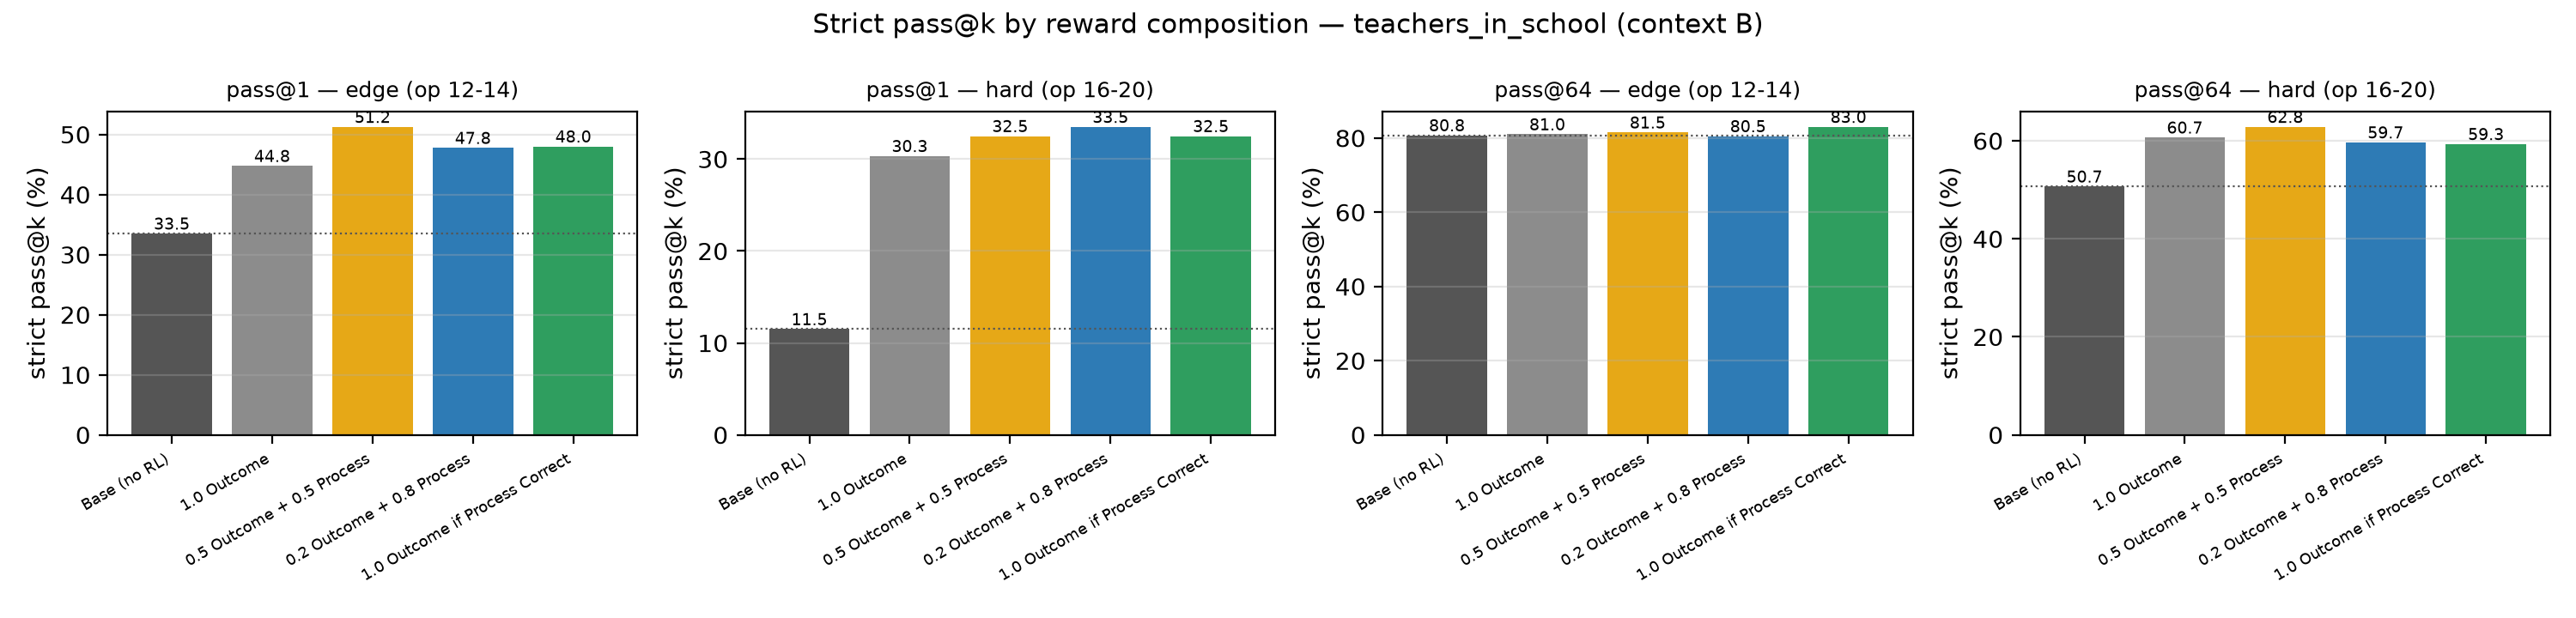
\includegraphics[width=\linewidth]{fig7_bars_teachers.png}
\caption{Strict \passk{1}/\passk{64} by reward composition and band, context B
(paper-Fig.~7 analogue). Dotted line: base model.}
\label{fig:fig7}
\end{figure}

\begin{figure}[t]
\centering
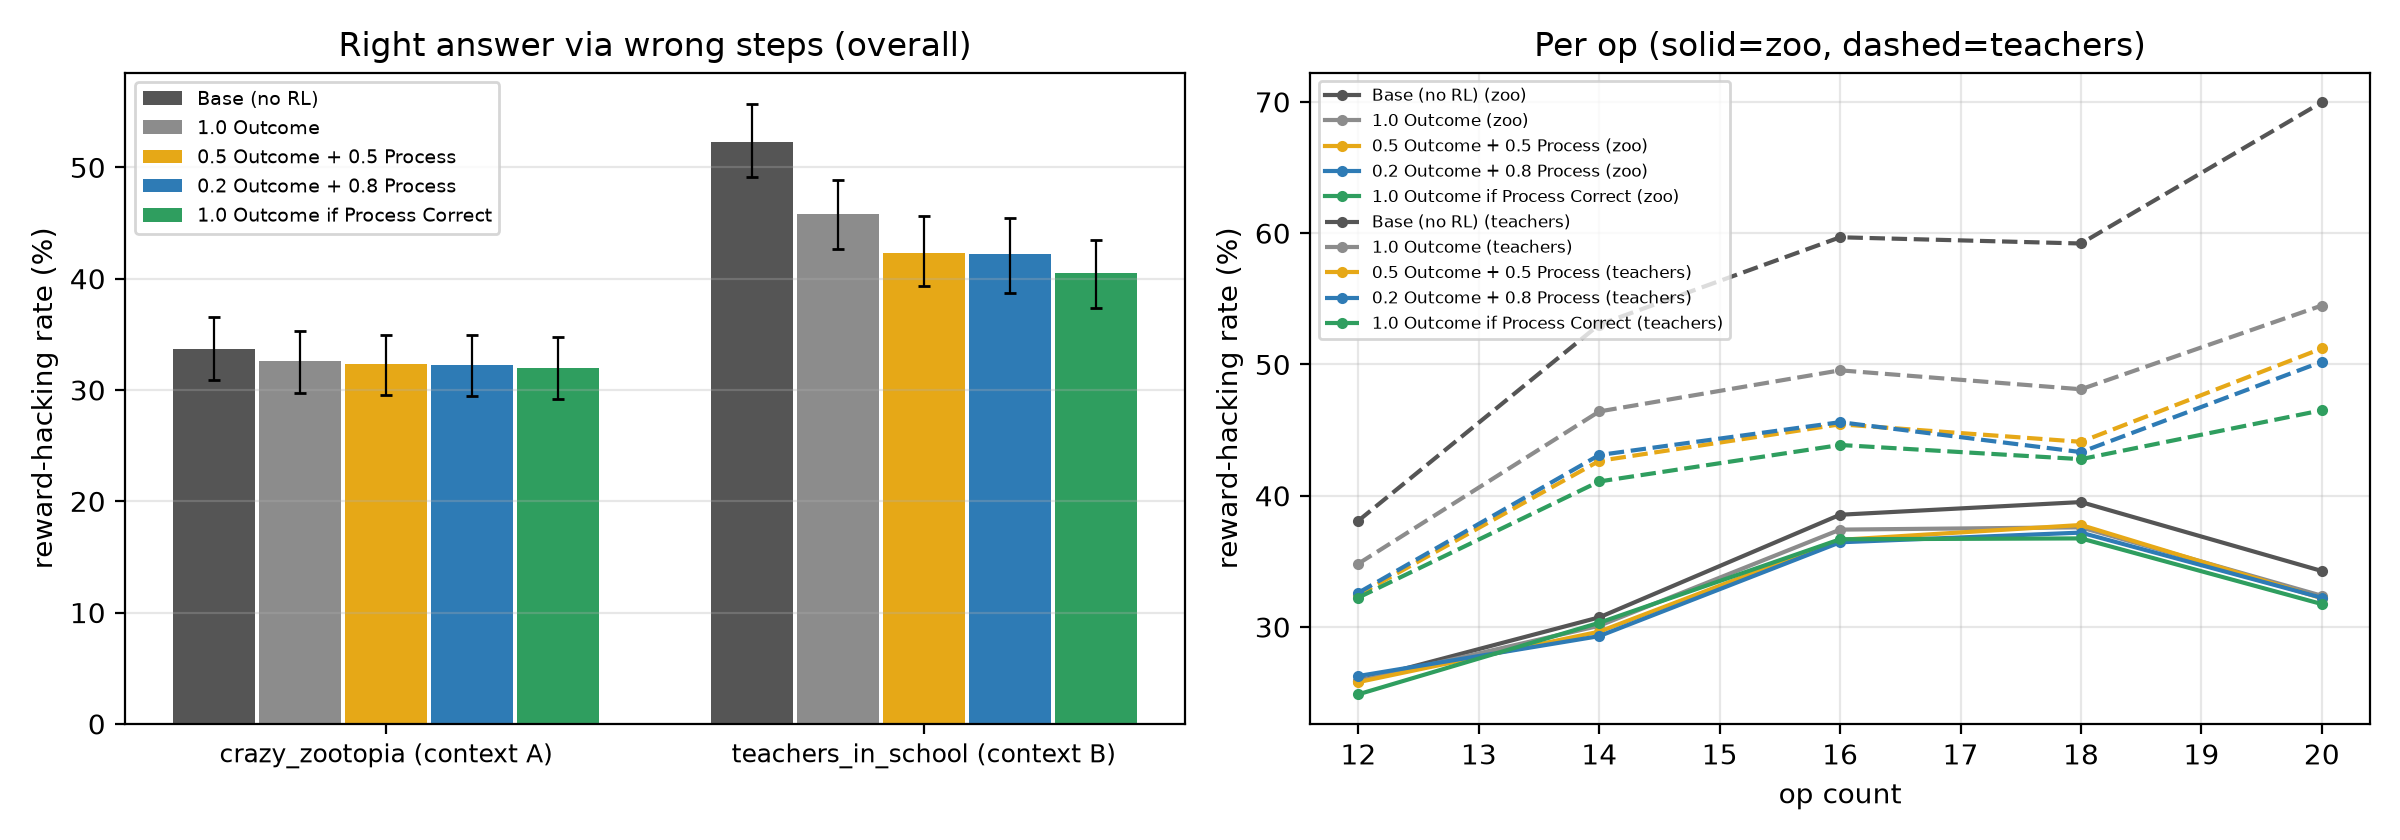
\includegraphics[width=\linewidth]{fig_hacking_rate.png}
\caption{Reward-hacking rate (Eq.~\ref{eq:hack}) by reward composition: overall per
context (left, with $95\%$ CIs) and per op count (right).}
\label{fig:hack}
\end{figure}

\section{Conclusions vs.\ the paper's predictions}

\begin{enumerate}[leftmargin=1.6em,itemsep=2pt]
\item \emph{``Any process signal raises strict \passk{1} by ${\sim}4$--$5$ points over
outcome-only on the hardest problems.''} --- \textbf{Directionally supported} on hard
($+2.2$ to $+3.2\pp$, sign-consistent, individually unresolved); \textbf{unambiguous on
edge} ($+6.5\pp$ \ci{+2.8}{+10.3}).
\item \emph{``0.2/0.8 and strict are best; strict has the lowest hacking rate.''} ---
\textbf{Confirmed under the released scorer} ($0.2/0.8$ best hard-band \passk{1};
hacking ladder Bonferroni-robust at every step). Under the \emph{corrected} scorer
the process-vs-outcome reduction survives in full ($-4.5\pp$, $p<10^{-3}$) but
strict's uniqueness does not: the three process variants tie on hacking and the
dense mixes dominate strict on accuracy --- the reward ranking is
verifier-regime-dependent (\S\ref{sec:artifact}).
\item \emph{``Process rewards shift errors away from wrong dependencies and missing
steps.''} --- \textbf{Supported in aggregate}, with the strict-gating missing-step
nuance (\S3.3) and the fewer-not-different-errors mechanism.
\end{enumerate}

\section{Limitations}
One training run per reward variant (CIs quantify evaluation uncertainty only ---
seed variance cannot be excluded; the paper shares this limitation). The paper ran
\S6 on extrapolation; the released reward variants exist only in the context setting
(directional comparability). The scorer artifact (\S\ref{sec:artifact}) biases
absolute strict metrics for all systems; we report orderings and paired differences,
which are robust. The outcome checkpoint's reward is answer-only (verified from its released config);
the 0.5/0.5 checkpoint's exact weights remain assumed. $k{=}64$ rather than the
paper's $128$, to fit a $3$-hour single-GPU budget.

\section{Reproducibility}
One command on PACE (\texttt{sbatch scripts/run\_all\_pace.sbatch}); pinned
environment (vLLM $0.10.1.1$, transformers $4.55.2$, torch $2.7.1$). Raw per-sample
outputs in \texttt{results/}; metrics, figures, and the four-audit validation
(clean-room recomputation, paired statistics with seed $12345$, $48$ annotated
qualitative cases, artifact re-scoring) in \texttt{analysis/}. Total compute:
$1$\,h\,$20$\,m on one H100.

\end{document}
